\documentclass[a4paper, 11pt]{article}
\usepackage{comment} % enables the use of multi-line comments (\ifx \fi) 
\usepackage{fullpage} % changes the margin
\usepackage[a4paper, total={7in, 10in}]{geometry}
\usepackage{amsmath,mathtools,mathdots,adjustbox,wrapfig}
\usepackage{amssymb,amsthm}  % assumes amsmath package installed
\usepackage{float}
\usepackage{xcolor}
\usepackage{mdframed}
%\usepackage{subfig}
\usepackage[shortlabels]{enumitem}
\usepackage{indentfirst}
\usepackage{hyperref}
\hypersetup{
    colorlinks=true,
    linkcolor=doc!80,
    citecolor=myr,
    filecolor=myr,      
    urlcolor=doc!80,
    pdftitle={Assignment}, %%%%%%%%%%%%%%%%   WRITE ASSIGNMENT PDF NAME  %%%%%%%%%%%%%%%%%%%%
}
\usepackage[most,many,breakable]{tcolorbox}
\usepackage{tikz}
%\usepackage{caption}
\usepackage{mathpazo}
\usepackage[skip=0.333\baselineskip]{caption}
\usepackage{subcaption}
% Use the libertine package for the Libertine font
\usepackage{libertine}
\usepackage[libertine]{newtxmath}
\usepackage{libertine}
\usepackage{physics}
\usepackage[ruled,vlined,linesnumbered]{algorithm2e}
\usepackage{mathrsfs}
\usepackage{tikz-cd}
\usepackage{float}
\usepackage{pgfplots}
\definecolor{mytheorembg}{HTML}{F2F2F9}
\definecolor{mytheoremfr}{HTML}{00007B}
\definecolor{doc}{RGB}{0,60,110}
\definecolor{myg}{RGB}{56, 140, 70}
\definecolor{myb}{RGB}{45, 111, 177}
\definecolor{myr}{RGB}{199, 68, 64}

\usetikzlibrary{decorations.pathreplacing,angles,quotes,patterns}
\definecolor{mytheorembg}{HTML}{F2F2F9}
\definecolor{mytheoremfr}{HTML}{00007B}
\definecolor{doc}{RGB}{0,60,110}
\definecolor{myg}{RGB}{56, 140, 70}
\definecolor{myb}{RGB}{45, 111, 177}
\definecolor{myr}{RGB}{199, 68, 64}
\newcounter{problem}
\tcbuselibrary{theorems,skins,hooks}
\newtcbtheorem[use counter=problem]{problem}{Problem}
{%
	enhanced,
	breakable,
	colback = mytheorembg,
	frame hidden,
	boxrule = 0sp,
	borderline west = {2pt}{0pt}{mytheoremfr},
	arc=5pt,
	detach title,
	before upper = \tcbtitle\par\smallskip,
	coltitle = mytheoremfr,
	fonttitle = \bfseries\sffamily,
	description font = \mdseries,
	separator sign none,
	segmentation style={solid, mytheoremfr},
}
{p}

\newtheorem{lemma}{Lemma}
\renewenvironment{proof}{\noindent{\it \textbf{Proof:}}\hspace*{1em}}{\qed\bigskip\\}
% To give references for any problem use like this
% suppose the problem number is p3 then 2 options either 
% \hyperref[p:p3]{<text you want to use to hyperlink> \ref{p:p3}}
%                  or directly 
%                   \ref{p:p3}



%---------------------------------------
% BlackBoard Math Fonts :-
%---------------------------------------

%Captital Letters
\newcommand{\bbA}{\mathbb{A}}	\newcommand{\bbB}{\mathbb{B}}
\newcommand{\bbC}{\mathbb{C}}	\newcommand{\bbD}{\mathbb{D}}
\newcommand{\bbE}{\mathbb{E}}	\newcommand{\bbF}{\mathbb{F}}
\newcommand{\bbG}{\mathbb{G}}	\newcommand{\bbH}{\mathbb{H}}
\newcommand{\bbI}{\mathbb{I}}	\newcommand{\bbJ}{\mathbb{J}}
\newcommand{\bbK}{\mathbb{K}}	\newcommand{\bbL}{\mathbb{L}}
\newcommand{\bbM}{\mathbb{M}}	\newcommand{\bbN}{\mathbb{N}}
\newcommand{\bbO}{\mathbb{O}}	\newcommand{\bbP}{\mathbb{P}}
\newcommand{\bbQ}{\mathbb{Q}}	\newcommand{\bbR}{\mathbb{R}}
\newcommand{\bbS}{\mathbb{S}}	\newcommand{\bbT}{\mathbb{T}}
\newcommand{\bbU}{\mathbb{U}}	\newcommand{\bbV}{\mathbb{V}}
\newcommand{\bbW}{\mathbb{W}}	\newcommand{\bbX}{\mathbb{X}}
\newcommand{\bbY}{\mathbb{Y}}	\newcommand{\bbZ}{\mathbb{Z}}

%---------------------------------------
% MathCal Fonts :-
%---------------------------------------

%Captital Letters
\newcommand{\mcA}{\mathcal{A}}	\newcommand{\mcB}{\mathcal{B}}
\newcommand{\mcC}{\mathcal{C}}	\newcommand{\mcD}{\mathcal{D}}
\newcommand{\mcE}{\mathcal{E}}	\newcommand{\mcF}{\mathcal{F}}
\newcommand{\mcG}{\mathcal{G}}	\newcommand{\mcH}{\mathcal{H}}
\newcommand{\mcI}{\mathcal{I}}	\newcommand{\mcJ}{\mathcal{J}}
\newcommand{\mcK}{\mathcal{K}}	\newcommand{\mcL}{\mathcal{L}}
\newcommand{\mcM}{\mathcal{M}}	\newcommand{\mcN}{\mathcal{N}}
\newcommand{\mcO}{\mathcal{O}}	\newcommand{\mcP}{\mathcal{P}}
\newcommand{\mcQ}{\mathcal{Q}}	\newcommand{\mcR}{\mathcal{R}}
\newcommand{\mcS}{\mathcal{S}}	\newcommand{\mcT}{\mathcal{T}}
\newcommand{\mcU}{\mathcal{U}}	\newcommand{\mcV}{\mathcal{V}}
\newcommand{\mcW}{\mathcal{W}}	\newcommand{\mcX}{\mathcal{X}}
\newcommand{\mcY}{\mathcal{Y}}	\newcommand{\mcZ}{\mathcal{Z}}



%---------------------------------------
% Bold Math Fonts :-
%---------------------------------------

%Captital Letters
\newcommand{\bmA}{\boldsymbol{A}}	\newcommand{\bmB}{\boldsymbol{B}}
\newcommand{\bmC}{\boldsymbol{C}}	\newcommand{\bmD}{\boldsymbol{D}}
\newcommand{\bmE}{\boldsymbol{E}}	\newcommand{\bmF}{\boldsymbol{F}}
\newcommand{\bmG}{\boldsymbol{G}}	\newcommand{\bmH}{\boldsymbol{H}}
\newcommand{\bmI}{\boldsymbol{I}}	\newcommand{\bmJ}{\boldsymbol{J}}
\newcommand{\bmK}{\boldsymbol{K}}	\newcommand{\bmL}{\boldsymbol{L}}
\newcommand{\bmM}{\boldsymbol{M}}	\newcommand{\bmN}{\boldsymbol{N}}
\newcommand{\bmO}{\boldsymbol{O}}	\newcommand{\bmP}{\boldsymbol{P}}
\newcommand{\bmQ}{\boldsymbol{Q}}	\newcommand{\bmR}{\boldsymbol{R}}
\newcommand{\bmS}{\boldsymbol{S}}	\newcommand{\bmT}{\boldsymbol{T}}
\newcommand{\bmU}{\boldsymbol{U}}	\newcommand{\bmV}{\boldsymbol{V}}
\newcommand{\bmW}{\boldsymbol{W}}	\newcommand{\bmX}{\boldsymbol{X}}
\newcommand{\bmY}{\boldsymbol{Y}}	\newcommand{\bmZ}{\boldsymbol{Z}}
%Small Letters
\newcommand{\bma}{\boldsymbol{a}}	\newcommand{\bmb}{\boldsymbol{b}}
\newcommand{\bmc}{\boldsymbol{c}}	\newcommand{\bmd}{\boldsymbol{d}}
\newcommand{\bme}{\boldsymbol{e}}	\newcommand{\bmf}{\boldsymbol{f}}
\newcommand{\bmg}{\boldsymbol{g}}	\newcommand{\bmh}{\boldsymbol{h}}
\newcommand{\bmi}{\boldsymbol{i}}	\newcommand{\bmj}{\boldsymbol{j}}
\newcommand{\bmk}{\boldsymbol{k}}	\newcommand{\bml}{\boldsymbol{l}}
\newcommand{\bmm}{\boldsymbol{m}}	\newcommand{\bmn}{\boldsymbol{n}}
\newcommand{\bmo}{\boldsymbol{o}}	\newcommand{\bmp}{\boldsymbol{p}}
\newcommand{\bmq}{\boldsymbol{q}}	\newcommand{\bmr}{\boldsymbol{r}}
\newcommand{\bms}{\boldsymbol{s}}	\newcommand{\bmt}{\boldsymbol{t}}
\newcommand{\bmu}{\boldsymbol{u}}	\newcommand{\bmv}{\boldsymbol{v}}
\newcommand{\bmw}{\boldsymbol{w}}	\newcommand{\bmx}{\boldsymbol{x}}
\newcommand{\bmy}{\boldsymbol{y}}	\newcommand{\bmz}{\boldsymbol{z}}


%---------------------------------------
% Scr Math Fonts :-
%---------------------------------------

\newcommand{\sA}{{\mathscr{A}}}   \newcommand{\sB}{{\mathscr{B}}}
\newcommand{\sC}{{\mathscr{C}}}   \newcommand{\sD}{{\mathscr{D}}}
\newcommand{\sE}{{\mathscr{E}}}   \newcommand{\sF}{{\mathscr{F}}}
\newcommand{\sG}{{\mathscr{G}}}   \newcommand{\sH}{{\mathscr{H}}}
\newcommand{\sI}{{\mathscr{I}}}   \newcommand{\sJ}{{\mathscr{J}}}
\newcommand{\sK}{{\mathscr{K}}}   \newcommand{\sL}{{\mathscr{L}}}
\newcommand{\sM}{{\mathscr{M}}}   \newcommand{\sN}{{\mathscr{N}}}
\newcommand{\sO}{{\mathscr{O}}}   \newcommand{\sP}{{\mathscr{P}}}
\newcommand{\sQ}{{\mathscr{Q}}}   \newcommand{\sR}{{\mathscr{R}}}
\newcommand{\sS}{{\mathscr{S}}}   \newcommand{\sT}{{\mathscr{T}}}
\newcommand{\sU}{{\mathscr{U}}}   \newcommand{\sV}{{\mathscr{V}}}
\newcommand{\sW}{{\mathscr{W}}}   \newcommand{\sX}{{\mathscr{X}}}
\newcommand{\sY}{{\mathscr{Y}}}   \newcommand{\sZ}{{\mathscr{Z}}}


%---------------------------------------
% Math Fraktur Font
%---------------------------------------

%Captital Letters
\newcommand{\mfA}{\mathfrak{A}}	\newcommand{\mfB}{\mathfrak{B}}
\newcommand{\mfC}{\mathfrak{C}}	\newcommand{\mfD}{\mathfrak{D}}
\newcommand{\mfE}{\mathfrak{E}}	\newcommand{\mfF}{\mathfrak{F}}
\newcommand{\mfG}{\mathfrak{G}}	\newcommand{\mfH}{\mathfrak{H}}
\newcommand{\mfI}{\mathfrak{I}}	\newcommand{\mfJ}{\mathfrak{J}}
\newcommand{\mfK}{\mathfrak{K}}	\newcommand{\mfL}{\mathfrak{L}}
\newcommand{\mfM}{\mathfrak{M}}	\newcommand{\mfN}{\mathfrak{N}}
\newcommand{\mfO}{\mathfrak{O}}	\newcommand{\mfP}{\mathfrak{P}}
\newcommand{\mfQ}{\mathfrak{Q}}	\newcommand{\mfR}{\mathfrak{R}}
\newcommand{\mfS}{\mathfrak{S}}	\newcommand{\mfT}{\mathfrak{T}}
\newcommand{\mfU}{\mathfrak{U}}	\newcommand{\mfV}{\mathfrak{V}}
\newcommand{\mfW}{\mathfrak{W}}	\newcommand{\mfX}{\mathfrak{X}}
\newcommand{\mfY}{\mathfrak{Y}}	\newcommand{\mfZ}{\mathfrak{Z}}
%Small Letters
\newcommand{\mfa}{\mathfrak{a}}	\newcommand{\mfb}{\mathfrak{b}}
\newcommand{\mfc}{\mathfrak{c}}	\newcommand{\mfd}{\mathfrak{d}}
\newcommand{\mfe}{\mathfrak{e}}	\newcommand{\mff}{\mathfrak{f}}
\newcommand{\mfg}{\mathfrak{g}}	\newcommand{\mfh}{\mathfrak{h}}
\newcommand{\mfi}{\mathfrak{i}}	\newcommand{\mfj}{\mathfrak{j}}
\newcommand{\mfk}{\mathfrak{k}}	\newcommand{\mfl}{\mathfrak{l}}
\newcommand{\mfm}{\mathfrak{m}}	\newcommand{\mfn}{\mathfrak{n}}
\newcommand{\mfo}{\mathfrak{o}}	\newcommand{\mfp}{\mathfrak{p}}
\newcommand{\mfq}{\mathfrak{q}}	\newcommand{\mfr}{\mathfrak{r}}
\newcommand{\mfs}{\mathfrak{s}}	\newcommand{\mft}{\mathfrak{t}}
\newcommand{\mfu}{\mathfrak{u}}	\newcommand{\mfv}{\mathfrak{v}}
\newcommand{\mfw}{\mathfrak{w}}	\newcommand{\mfx}{\mathfrak{x}}
\newcommand{\mfy}{\mathfrak{y}}	\newcommand{\mfz}{\mathfrak{z}}

%---------------------------------------
% Bar
%---------------------------------------

%Captital Letters
\newcommand{\ovA}{\overline{A}}	\newcommand{\ovB}{\overline{B}}
\newcommand{\ovC}{\overline{C}}	\newcommand{\ovD}{\overline{D}}
\newcommand{\ovE}{\overline{E}}	\newcommand{\ovF}{\overline{F}}
\newcommand{\ovG}{\overline{G}}	\newcommand{\ovH}{\overline{H}}
\newcommand{\ovI}{\overline{I}}	\newcommand{\ovJ}{\overline{J}}
\newcommand{\ovK}{\overline{K}}	\newcommand{\ovL}{\overline{L}}
\newcommand{\ovM}{\overline{M}}	\newcommand{\ovN}{\overline{N}}
\newcommand{\ovO}{\overline{O}}	\newcommand{\ovP}{\overline{P}}
\newcommand{\ovQ}{\overline{Q}}	\newcommand{\ovR}{\overline{R}}
\newcommand{\ovS}{\overline{S}}	\newcommand{\ovT}{\overline{T}}
\newcommand{\ovU}{\overline{U}}	\newcommand{\ovV}{\overline{V}}
\newcommand{\ovW}{\overline{W}}	\newcommand{\ovX}{\overline{X}}
\newcommand{\ovY}{\overline{Y}}	\newcommand{\ovZ}{\overline{Z}}
%Small Letters
\newcommand{\ova}{\overline{a}}	\newcommand{\ovb}{\overline{b}}
\newcommand{\ovc}{\overline{c}}	\newcommand{\ovd}{\overline{d}}
\newcommand{\ove}{\overline{e}}	\newcommand{\ovf}{\overline{f}}
\newcommand{\ovg}{\overline{g}}	\newcommand{\ovh}{\overline{h}}
\newcommand{\ovi}{\overline{i}}	\newcommand{\ovj}{\overline{j}}
\newcommand{\ovk}{\overline{k}}	\newcommand{\ovl}{\overline{l}}
\newcommand{\ovm}{\overline{m}}	\newcommand{\ovn}{\overline{n}}
\newcommand{\ovo}{\overline{o}}	\newcommand{\ovp}{\overline{p}}
\newcommand{\ovq}{\overline{q}}	\newcommand{\ovr}{\overline{r}}
\newcommand{\ovs}{\overline{s}}	\newcommand{\ovt}{\overline{t}}
\newcommand{\ovu}{\overline{u}}	\newcommand{\ovv}{\overline{v}}
\newcommand{\ovw}{\overline{w}}	\newcommand{\ovx}{\overline{x}}
\newcommand{\ovy}{\overline{y}}	\newcommand{\ovz}{\overline{z}}

%---------------------------------------
% Tilde
%---------------------------------------

%Captital Letters
\newcommand{\tdA}{\tilde{A}}	\newcommand{\tdB}{\tilde{B}}
\newcommand{\tdC}{\tilde{C}}	\newcommand{\tdD}{\tilde{D}}
\newcommand{\tdE}{\tilde{E}}	\newcommand{\tdF}{\tilde{F}}
\newcommand{\tdG}{\tilde{G}}	\newcommand{\tdH}{\tilde{H}}
\newcommand{\tdI}{\tilde{I}}	\newcommand{\tdJ}{\tilde{J}}
\newcommand{\tdK}{\tilde{K}}	\newcommand{\tdL}{\tilde{L}}
\newcommand{\tdM}{\tilde{M}}	\newcommand{\tdN}{\tilde{N}}
\newcommand{\tdO}{\tilde{O}}	\newcommand{\tdP}{\tilde{P}}
\newcommand{\tdQ}{\tilde{Q}}	\newcommand{\tdR}{\tilde{R}}
\newcommand{\tdS}{\tilde{S}}	\newcommand{\tdT}{\tilde{T}}
\newcommand{\tdU}{\tilde{U}}	\newcommand{\tdV}{\tilde{V}}
\newcommand{\tdW}{\tilde{W}}	\newcommand{\tdX}{\tilde{X}}
\newcommand{\tdY}{\tilde{Y}}	\newcommand{\tdZ}{\tilde{Z}}
%Small Letters
\newcommand{\tda}{\tilde{a}}	\newcommand{\tdb}{\tilde{b}}
\newcommand{\tdc}{\tilde{c}}	\newcommand{\tdd}{\tilde{d}}
\newcommand{\tde}{\tilde{e}}	\newcommand{\tdf}{\tilde{f}}
\newcommand{\tdg}{\tilde{g}}	\newcommand{\tdh}{\tilde{h}}
\newcommand{\tdi}{\tilde{i}}	\newcommand{\tdj}{\tilde{j}}
\newcommand{\tdk}{\tilde{k}}	\newcommand{\tdl}{\tilde{l}}
\newcommand{\tdm}{\tilde{m}}	\newcommand{\tdn}{\tilde{n}}
\newcommand{\tdo}{\tilde{o}}	\newcommand{\tdp}{\tilde{p}}
\newcommand{\tdq}{\tilde{q}}	\newcommand{\tdr}{\tilde{r}}
\newcommand{\tds}{\tilde{s}}	\newcommand{\tdt}{\tilde{t}}
\newcommand{\tdu}{\tilde{u}}	\newcommand{\tdv}{\tilde{v}}
\newcommand{\tdw}{\tilde{w}}	\newcommand{\tdx}{\tilde{x}}
\newcommand{\tdy}{\tilde{y}}	\newcommand{\tdz}{\tilde{z}}

%---------------------------------------
% Vec
%---------------------------------------

%Captital Letters
\newcommand{\vcA}{\vec{A}}	\newcommand{\vcB}{\vec{B}}
\newcommand{\vcC}{\vec{C}}	\newcommand{\vcD}{\vec{D}}
\newcommand{\vcE}{\vec{E}}	\newcommand{\vcF}{\vec{F}}
\newcommand{\vcG}{\vec{G}}	\newcommand{\vcH}{\vec{H}}
\newcommand{\vcI}{\vec{I}}	\newcommand{\vcJ}{\vec{J}}
\newcommand{\vcK}{\vec{K}}	\newcommand{\vcL}{\vec{L}}
\newcommand{\vcM}{\vec{M}}	\newcommand{\vcN}{\vec{N}}
\newcommand{\vcO}{\vec{O}}	\newcommand{\vcP}{\vec{P}}
\newcommand{\vcQ}{\vec{Q}}	\newcommand{\vcR}{\vec{R}}
\newcommand{\vcS}{\vec{S}}	\newcommand{\vcT}{\vec{T}}
\newcommand{\vcU}{\vec{U}}	\newcommand{\vcV}{\vec{V}}
\newcommand{\vcW}{\vec{W}}	\newcommand{\vcX}{\vec{X}}
\newcommand{\vcY}{\vec{Y}}	\newcommand{\vcZ}{\vec{Z}}
%Small Letters
\newcommand{\vca}{\vec{a}}	\newcommand{\vcb}{\vec{b}}
\newcommand{\vcc}{\vec{c}}	\newcommand{\vcd}{\vec{d}}
\newcommand{\vce}{\vec{e}}	\newcommand{\vcf}{\vec{f}}
\newcommand{\vcg}{\vec{g}}	\newcommand{\vch}{\vec{h}}
\newcommand{\vci}{\vec{i}}	\newcommand{\vcj}{\vec{j}}
\newcommand{\vck}{\vec{k}}	\newcommand{\vcl}{\vec{l}}
\newcommand{\vcm}{\vec{m}}	\newcommand{\vcn}{\vec{n}}
\newcommand{\vco}{\vec{o}}	\newcommand{\vcp}{\vec{p}}
\newcommand{\vcq}{\vec{q}}	\newcommand{\vcr}{\vec{r}}
\newcommand{\vcs}{\vec{s}}	\newcommand{\vct}{\vec{t}}
\newcommand{\vcu}{\vec{u}}	\newcommand{\vcv}{\vec{v}}
%\newcommand{\vcw}{\vec{w}}	\newcommand{\vcx}{\vec{x}}
\newcommand{\vcy}{\vec{y}}	\newcommand{\vcz}{\vec{z}}

%---------------------------------------
% Greek Letters:-
%---------------------------------------
\newcommand{\eps}{\epsilon}
\newcommand{\veps}{\varepsilon}
\newcommand{\lm}{\lambda}
\newcommand{\Lm}{\Lambda}
\newcommand{\gm}{\gamma}
\newcommand{\Gm}{\Gamma}
\newcommand{\vph}{\varphi}
\newcommand{\ph}{\phi}
\newcommand{\om}{\omega}
\newcommand{\Om}{\Omega}
\newcommand{\sg}{\sigma}
\newcommand{\Sg}{\Sigma}

\newcommand{\Qed}{\begin{flushright}\qed\end{flushright}}
\newcommand{\parinn}{\setlength{\parindent}{1cm}}
\newcommand{\parinf}{\setlength{\parindent}{0cm}}
\newcommand{\del}[2]{\frac{\partial #1}{\partial #2}}
\newcommand{\Del}[3]{\frac{\partial^{#1} #2}{\partial^{#1} #3}}
\newcommand{\deld}[2]{\dfrac{\partial #1}{\partial #2}}
\newcommand{\Deld}[3]{\dfrac{\partial^{#1} #2}{\partial^{#1} #3}}
\newcommand{\uin}{\mathbin{\rotatebox[origin=c]{90}{$\in$}}}
\newcommand{\usubset}{\mathbin{\rotatebox[origin=c]{90}{$\subset$}}}
\newcommand{\lt}{\left}
\newcommand{\rt}{\right}
\newcommand{\exs}{\exists}
\newcommand{\st}{\strut}
\newcommand{\dps}[1]{\displaystyle{#1}}
\newcommand{\la}{\langle}
\newcommand{\ra}{\rangle}
\newcommand{\cls}[1]{\textsc{#1}}
\newcommand{\prb}[1]{\textsc{#1}}
\newcommand{\comb}[2]{\left(\begin{matrix}
		#1\\ #2
\end{matrix}\right)}
%\newcommand[2]{\quotient}{\faktor{#1}{#2}}
\newcommand\quotient[2]{
	\mathchoice
	{% \displaystyle
		\text{\raise1ex\hbox{$#1$}\Big/\lower1ex\hbox{$#2$}}%
	}
	{% \textstyle
		#1\,/\,#2
	}
	{% \scriptstyle
		#1\,/\,#2
	}
	{% \scriptscriptstyle  
		#1\,/\,#2
	}
}

\newcommand{\tensor}{\otimes}
\newcommand{\xor}{\oplus}

\newcommand{\sol}[1]{\begin{solution}#1\end{solution}}
\newcommand{\solve}[1]{\setlength{\parindent}{0cm}\textbf{\textit{Solution: }}\setlength{\parindent}{1cm}#1 \hfill $\blacksquare$}
\newcommand{\mat}[1]{\left[\begin{matrix}#1\end{matrix}\right]}
\newcommand{\matr}[1]{\begin{matrix}#1\end{matrix}}
\newcommand{\matp}[1]{\lt(\begin{matrix}#1\end{matrix}\rt)}
\newcommand{\detmat}[1]{\lt|\begin{matrix}#1\end{matrix}\rt|}
\newcommand\numberthis{\addtocounter{equation}{1}\tag{\theequation}}
\newcommand{\handout}[3]{
	\noindent
	\begin{center}
		\framebox{
			\vbox{
				\hbox to 6.5in { {\bf Complexity Theory I } \hfill Jan -- May, 2023 }
				\vspace{4mm}
				\hbox to 6.5in { {\Large \hfill #1  \hfill} }
				\vspace{2mm}
				\hbox to 6.5in { {\em #2 \hfill #3} }
			}
		}
	\end{center}
	\vspace*{4mm}
}

\newcommand{\lecture}[3]{\handout{Lecture #1}{Lecturer: #2}{Scribe:	#3}}

\let\marvosymLightning\Lightning
\newcommand{\ctr}{\text{\marvosymLightning}\hspace{0.5ex}} % Requires marvosym package

\newcommand{\ov}[1]{\overline{#1}}
\newcommand{\thmref}[1]{\hyperref[th:#1]{Theorem \ref{th:#1}}}
\newcommand{\propref}[1]{\hyperref[th:#1]{Proposition \ref{th:#1}}}
\newcommand{\lmref}[1]{\hyperref[th:#1]{Lemma \ref{th:#1}}}
\newcommand{\corref}[1]{\hyperref[th:#1]{Corollary \ref{th:#1}}}

\newcommand{\thrmref}[1]{\hyperref[#1]{Theorem \ref{#1}}}
\newcommand{\propnref}[1]{\hyperref[#1]{Proposition \ref{#1}}}
\newcommand{\lemref}[1]{\hyperref[#1]{Lemma \ref{#1}}}
\newcommand{\corrref}[1]{\hyperref[#1]{Corollary \ref{#1}}}

\DeclareMathOperator{\enc}{Enc}
\DeclareMathOperator{\res}{Res}
\DeclareMathOperator{\spec}{Spec}
\DeclareMathOperator{\cov}{Cov}
\DeclareMathOperator{\Var}{Var}
\DeclareMathOperator{\Rank}{rank}
\newcommand{\Tfae}{The following are equivalent:}
\newcommand{\tfae}{the following are equivalent:}
\newcommand{\sparsity}{\textit{sparsity}}

\newcommand{\uddots}{\reflectbox{$\ddots$}} 

\newenvironment{claimwidth}{\begin{center}\begin{adjustwidth}{0.05\textwidth}{0.05\textwidth}}{\end{adjustwidth}\end{center}}

\setlength{\parindent}{0pt}

%%%%%%%%%%%%%%%%%%%%%%%%%%%%%%%%%%%%%%%%%%%%%%%%%%%%%%%%%%%%%%%%%%%%%%%%%%%%%%%%%%%%%%%%%%%%%%%%%%%%%%%%%%%%%%%%%%%%%%%%%%%%%%%%%%%%%%%%

\begin{document}

%%%%%%%%%%%%%%%%%%%%%%%%%%%%%%%%%%%%%%%%%%%%%%%%%%%%%%%%%%%%%%%%%%%%%%%%%%%%%%%%%%%%%%%%%%%%%%%%%%%%%%%%%%%%%%%%%%%%%%%%%%%%%%%%%%%%%%%%

\textsf{\noindent \large\textbf{Soham Chatterjee} \hfill \textbf{Assignment - 5}\\
    Email: \href{soham.chatterjee@tifr.res.in}{soham.chatterjee@tifr.res.in} \hfill Dept: STCS\\
    \normalsize Course: Probability Theory \hfill Date: \today
    \\  \noindent\rule{7in}{2.8pt}
}

[All the problems I discussed with Spandan, Soumyadeep]
%%%%%%%%%%%%%%%%%%%%%%%%%%%%%%%%%%%%%%%%%%%%%%%%%%%%%%%%%%%%%%%%%%%%%%%%%%%%%%%%%%%%%%%%%%%%%%%%%%%%%%%%%%%%%%%%%%%%%%%%%%%%%%%%%%%%%%%%
% Problem 1
%%%%%%%%%%%%%%%%%%%%%%%%%%%%%%%%%%%%%%%%%%%%%%%%%%%%%%%%%%%%%%%%%%%%%%%%%%%%%%%%%%%%%%%%%%%%%%%%%%%%%%%%%%%%%%%%%%%%%%%%%%%%%%%%%%%%%%%%

\begin{problem}{%problem statement
    }{p1% problem reference text
    }
Let $X,Y_1,Y_2$ be three random variables with joint density $f_{X,Y_1,Y_2}$. For a fixed $y_1$, consider two random variables $\tilde{X}$, $\tilde{Y_2}$ with joint distribution $g_{\tdX,\tilde{Y_2}}$ defined as $g_{\tdX,\tilde{Y_2}}(x,y_2)=f_{X,Y_2\mid Y_1}(x,y_2\mid y_1)$. Show that $$\bbE[\tdX\mid \tdY=y_2]=\bbE[X\mid Y_1=y_1,Y_2=y_2]$$What is the relevance of this fact in our derivation of recursive estimation in the lecture?
\end{problem}
\solve{
We have $$g_{\tdX\mid \tdY_2}(x\mid y_2)=\frac{g_{\tdX,\tdY_2}(x,y_2)}{g_{\tdY_2}(y_2)}=\frac{f_{X,Y_2\mid Y_1}(x,y_2\mid y_1)}{f_{Y_2\mid Y_1}(y_2\mid y_1)}=\frac{\frac{f_{X,Y_1,Y_2}(x,y_1,y_2)}{f_{Y_1}(y_1)}}{\frac{f_{Y_1,Y_2}(y_1,y_2)}{f_{Y_1}(y_1)}}=f_{X\mid Y_1,Y_2}(x\mid y_1,y_2)$$Therefore $\bbE[\tdX\mid \tdY=y_2]=\bbE[X\mid Y_1=y_1,Y_2=y_2]$. This is used to derive the iterative estimator which is used in the recurrence relation for Kalman Filter.
}
%%%%%%%%%%%%%%%%%%%%%%%%%%%%%%%%%%%%%%%%%%%%%%%%%%%%%%%%%%%%%%%%%%%%%%%%%%%%%%%%%%%%%%%%%%%%%%%%%%%%%%%%%%%%%%%%%%%%%%%%%%%%%%%%%%%%%%%%
% Problem 2
%%%%%%%%%%%%%%%%%%%%%%%%%%%%%%%%%%%%%%%%%%%%%%%%%%%%%%%%%%%%%%%%%%%%%%%%%%%%%%%%%%%%%%%%%%%%%%%%%%%%%%%%%%%%%%%%%%%%%%%%%%%%%%%%%%%%%%%%

\begin{problem}{%problem statement
    }{p2% problem reference text
    }
Consider the Kalman filtering problem for the scalar system:

\begin{align*}
	X_k  =\alpha X_{k-1}+W_k && 	Y_k =h X_k+Z_k
\end{align*}
as described in class (i.e., $W_k \sim N\left(0, \sigma_W^2\right)$ i.i.d, $Z_k \sim N\left(0, \sigma_Z^2\right)$, and $X_1$ are independent). The initial condition is $X_1 \sim N\left(0, \sigma_{X_1}^2\right)$. For the numerical exercises below you can assume $\sigma_{X_1}^2=\sigma_Z^2=\sigma_W^2=h=1$.\begin{enumerate}[label=(\alph*)]
	\item Plot sample paths of the process $\left\{X_k\right\}$ for different values of $\alpha$. Pick a representative set of values of $\alpha$ to show the effect of $\alpha$ on how the sample paths look like. Can you explain qualitatively the effect?
\item Let $\hat{X}_k=E\left[X_k \mid Y_1, \ldots, Y_k\right]$. For those sample paths of $\left\{X_k\right\}$ plotted in part (a), plot in the same figure the sample paths of the estimates $\left\{\hat{X}_k\right\}$. What is the qualitative effect of $\alpha$ on the estimation errors?
\item Let $\tilde{X}_k=E\left[X_k \mid Y_k\right]$. This is the state estimate based only on the current observation. For the sample paths in (a) and (b), plot the sample paths of $\left\{\tilde{X}_k\right\}$ in the same figure as well. How does the difference in the accuracy of the estimators $\hat{X}_k$ and $\tilde{X}_k$ depend on the value of $\alpha$ ? Explain qualitatively.
\item Let $f_k$ be the conditional distribution of $X_k$ give the observations up to time $k$. For your favorite value of $\alpha$, plot $f_k$ for several values of $k$ to get a feel of how the distribution evolves in time. Do these distributions depend on the random outcome of the experiment? How?
\item What happens to the distribution of $X_k$ as $k \rightarrow \infty$ ? Give a quantitative answer. Does your answer depend on $\alpha$ ? Does your answer depend on $\sigma_{X_1}^2$ ?
\item What happens to the MMSE estimation error $\sigma_k^2$ of $\hat{X}_k$ as $k \rightarrow \infty$ ? Does it converge to zero, a finite non-zero value or infinity? How does your answer depend on $\alpha$ ? An answer supported by numerical evidence together with some analysis would be fine; it doesn't have to be totally rigorous.
\end{enumerate}
\end{problem}
\solve{
\begin{enumerate}[label=(\alph*)]
	\item Here we have taken the values of $\alpha$ to be $\{-1,0.8,1,1.2\}$ in \hyperref[fig:fig1]{Figure 1}. Here we can see that when the value of $\alpha$ is $1.2$  then the sample value increases. And when the value of $\alpha$ is $-1$ it oscillates around $0$. But for $\alpha=0.8$ the sample values remains close to $0$. Therefore the sample values converges when $|\alpha|<1$ and otherwise diverges.

	

\begin{figure}[hbt!]%
	\centering
	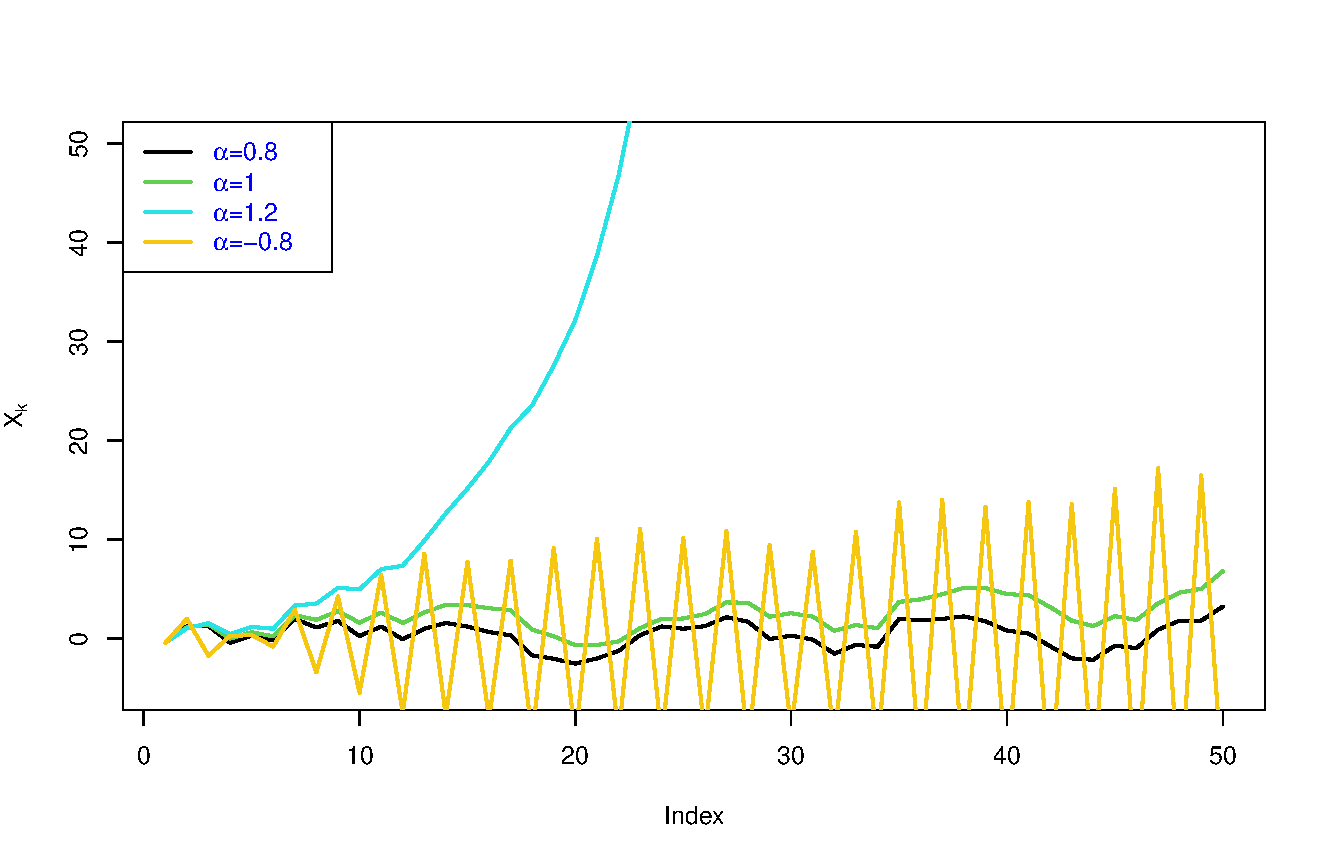
\includegraphics[width=8cm]{./ass5.2a.pdf}\label{fig:fig1}%
	\caption{Plot of $X_k$ for different $\alpha\in \{-1,0.8,1,1.2\}$}%
%	\label{fig:example}%
\end{figure}

\item In the  following plot we can see that the predicted values $\bbE[X\mid Y_1,\dots, Y_k]$ matches almost correctly with the sample values $X_k$. From the plots we conclude that as $|\alpha$ becomes larger it has lesser effect on the estimation which we also showed in part (f) where we showed if $|\alpha|$ becomes larger then the MMSE estimation is independent of $\alpha$. 

\begin{figure}[hbt!]
	\begin{subfigure}{.475\linewidth}
		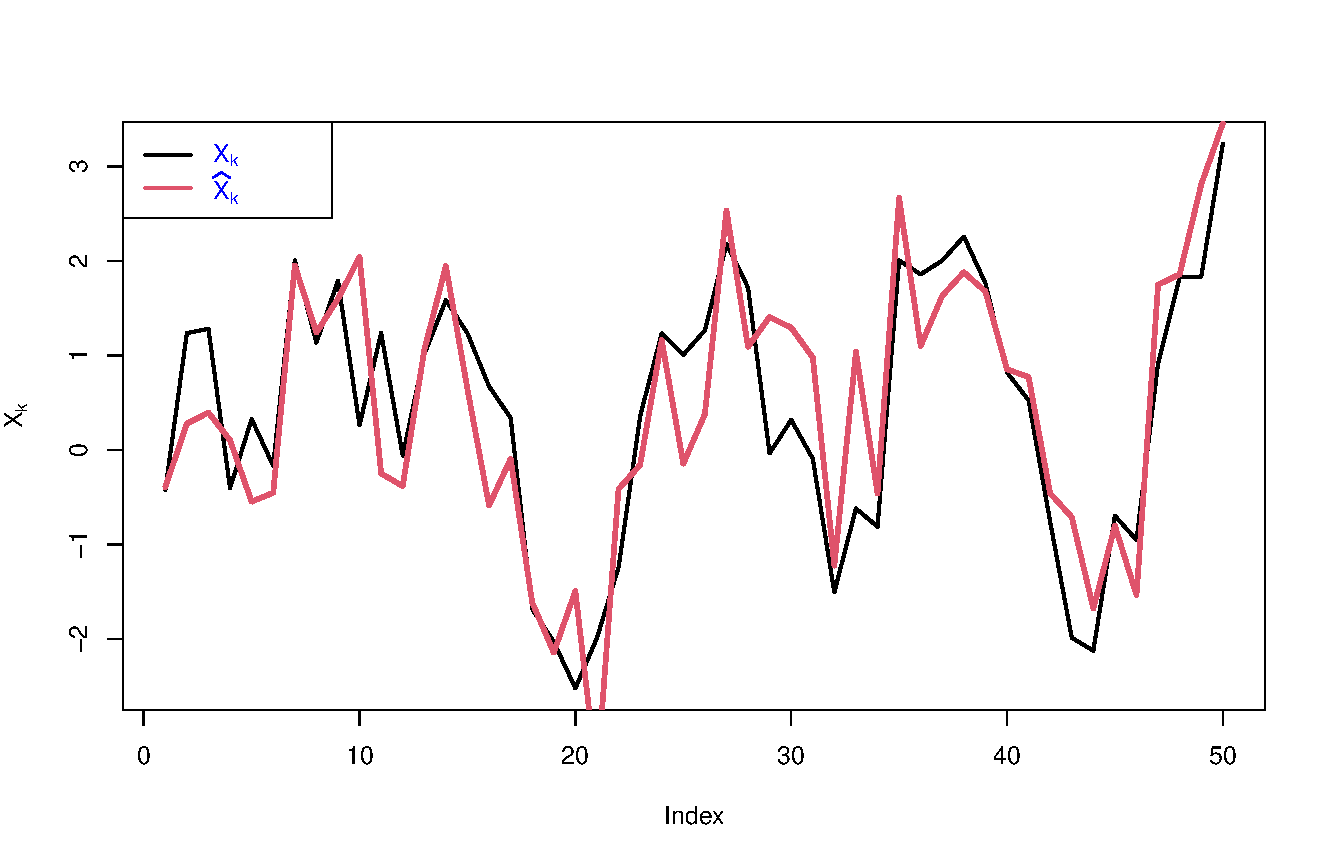
\includegraphics[width=\linewidth]{./ass5.2b-0.8.pdf}
		\caption{Plot of $X_k$ vs $\hat{X}_k$ for $\alpha=0.8$}
		\label{MLEDdet}
	\end{subfigure}\hfill % <-- "\hfill"
	\begin{subfigure}{.475\linewidth}
		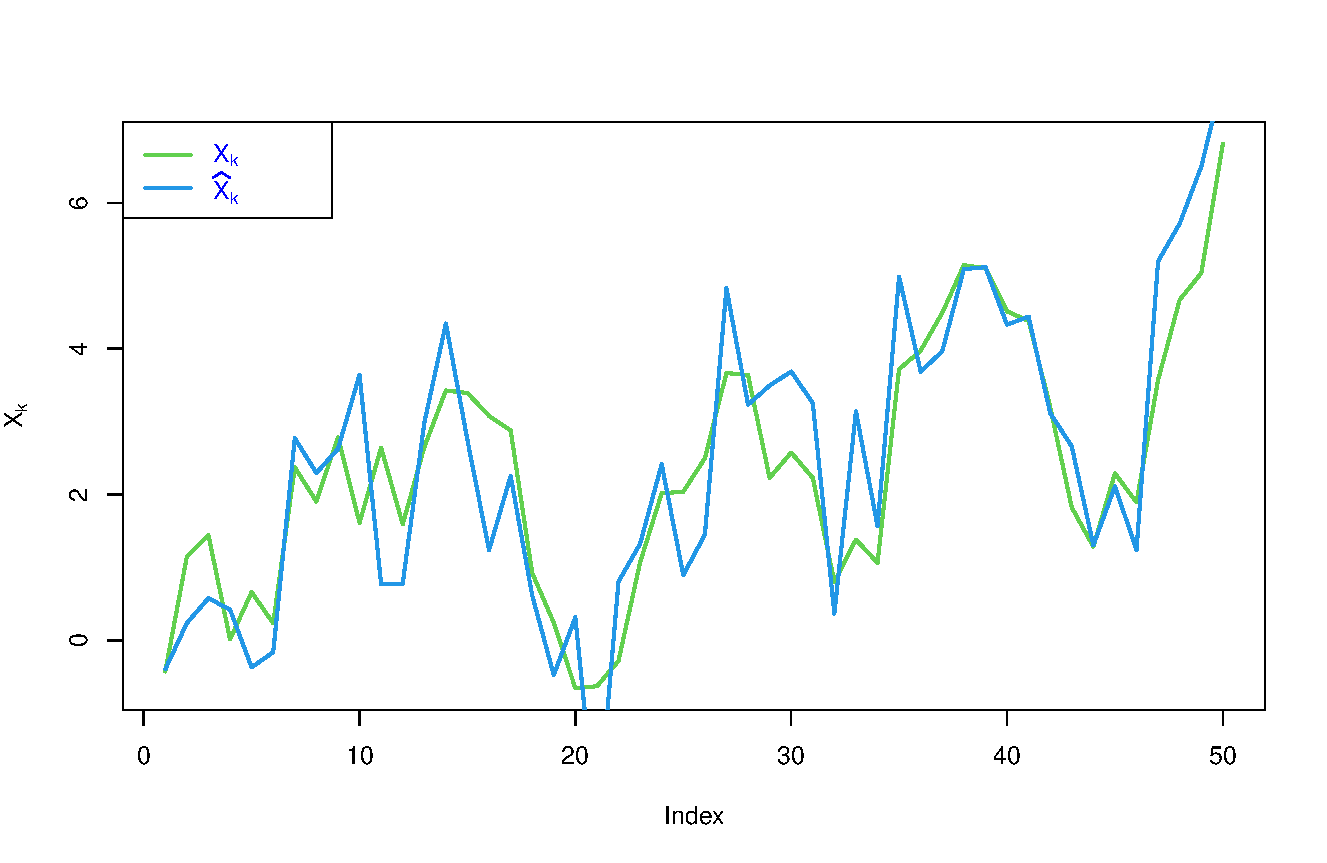
\includegraphics[width=\linewidth]{./ass5.2b-1.pdf}
		\caption{Plot of $X_k$ vs $\hat{X}_k$ for $\alpha=1$}
		\label{energydetPSK}
	\end{subfigure}
	
	\medskip % create some *vertical* separation between the graphs
	\begin{subfigure}{.475\linewidth}
		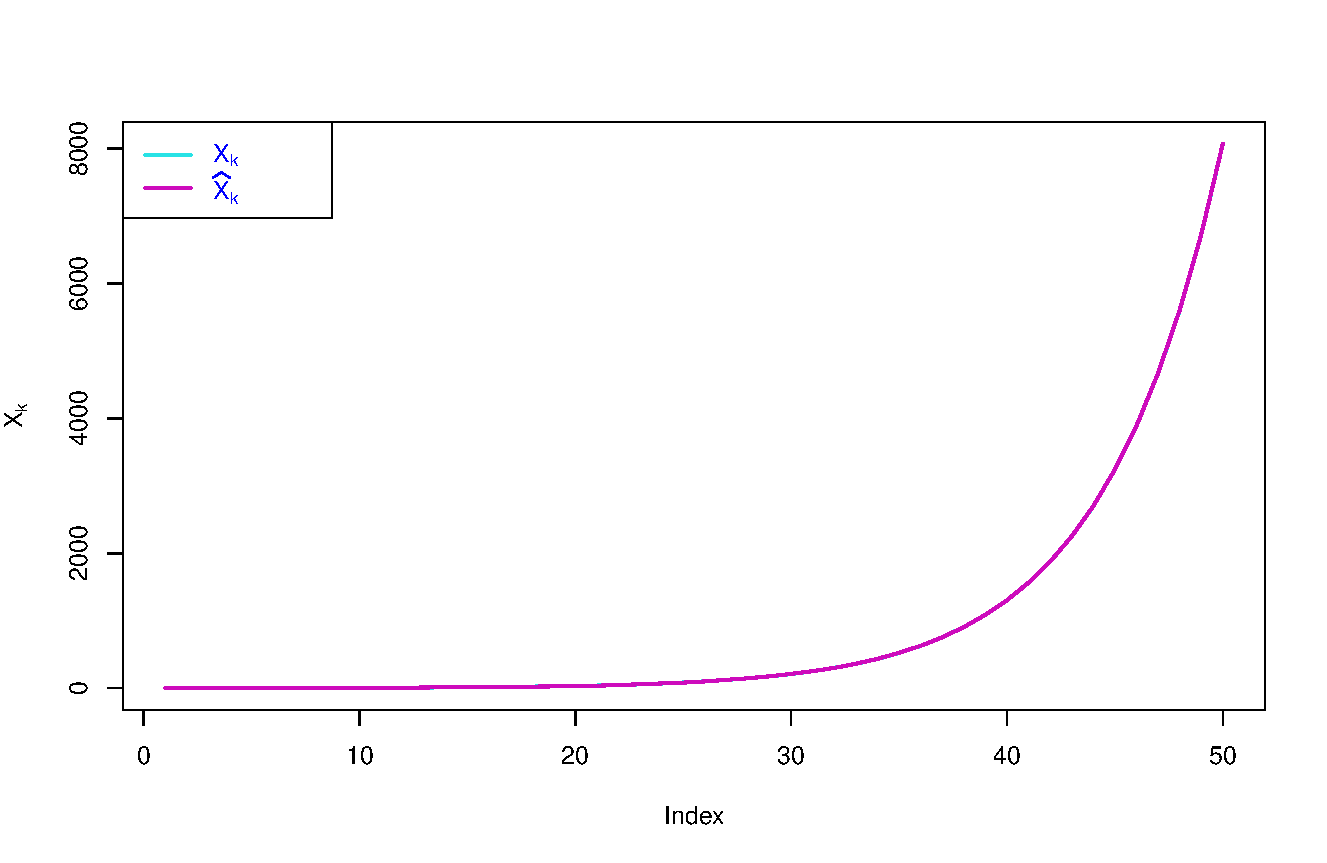
\includegraphics[width=\linewidth]{./ass5.2b-1.2.pdf}
		\caption{Plot of $X_k$ vs $\hat{X}_k$ for $\alpha=1.2$}
		\label{velcomp}
	\end{subfigure}\hfill % <-- "\hfill"
	\begin{subfigure}{.475\linewidth}
		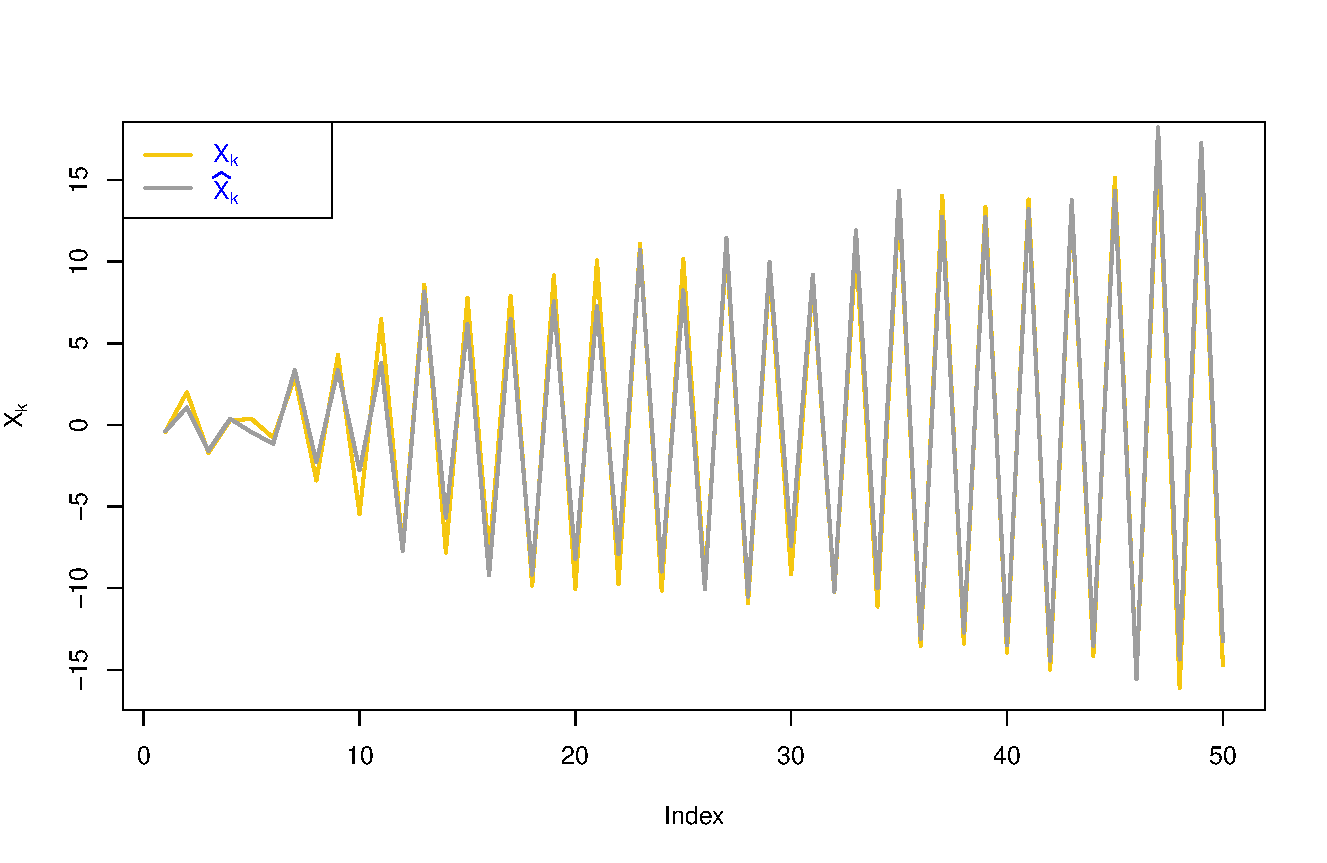
\includegraphics[width=\linewidth]{./ass5.2b--1.pdf}
		\caption{Plot of $X_k$ vs $\hat{X}_k$ for $\alpha=-1$}
		\label{estcomp}
	\end{subfigure}
	
	\caption{Compared $X_k$ and predicted $\hat{X_k}$}
	\label{fig:roc}
\end{figure}



\item Here we compare $X_k$, $\hat{S}_k$ and $\tdX_k=\bbE[X_k\mid Y_k]$ for all values of $\alpha$. Now we have $\cov(X_k,Y_k)=h\rho_k^2$ and $\Var[Y_k]=h^2\rho_k^2+\sg_Z^2$. Hence we have $$\bbE[X_k\mid Y_k]=\frac{h\rho_k^2 Y_k}{h^2\rho_k^2+\sg_Z^2}$$So we have\begin{align*}
	\bbE[X_k-\tdX_k]^2 & = \bbE\lt[X_k-\frac{h\rho_k^2 Y_k}{h^2\rho_k^2+\sg_Z^2}\rt] ^2\\
	& = \frac{1}{\lt(h^2\rho_k^2+\sg_Z^2\rt)^2}\bbE\lt[(h^2\rho_k^2+\sg_Z^2)X_k-h\rho_k^2(hX_k+Z_k)\rt]^2\\
	& = \frac{1}{\lt(h^2\rho_k^2+\sg_Z^2\rt)^2}\bbE[\sg_Z^2X_k-h\rho_k^2Z_k]^2\\
	& = \frac{\sg_Z^4\rho_k^2+h^2\rho_k^4\sg_Z^2}{\lt(h^2\rho_k^2+\sg_Z^2\rt)^2}= \frac{\sg_Z^2\rho_k^2}{h^2\rho_k^2+\sg_Z^2}
\end{align*}Now this is the MMSE estimation of $\sg_k^2$ of $X_k$ which comparing with part (f) we can see that we obtained the same estimation value. Therefore both $\hat{X}_k$ and $\tdX_k$ are equally good estimating sample values. 

\begin{figure}[hbt!]
\begin{subfigure}{.475\linewidth}
	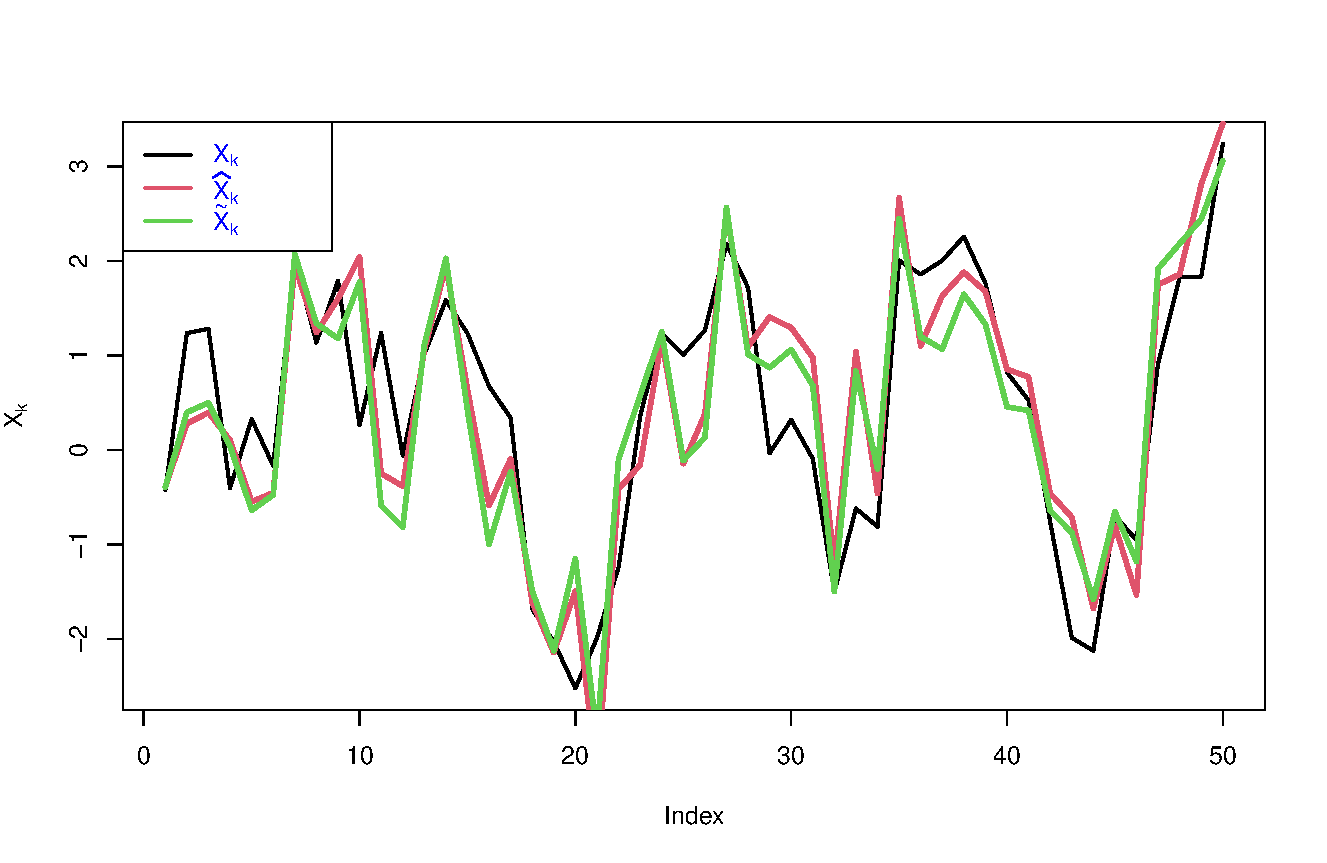
\includegraphics[width=\linewidth]{./ass5.2c-0.8.pdf}
	\caption{Plot of $X_k$ vs $\hat{X}_k$ vs $\tilde{X}_k$ for $\alpha=0.8$}
	\label{MLEDdet}
\end{subfigure}\hfill % <-- "\hfill"
\begin{subfigure}{.475\linewidth}
	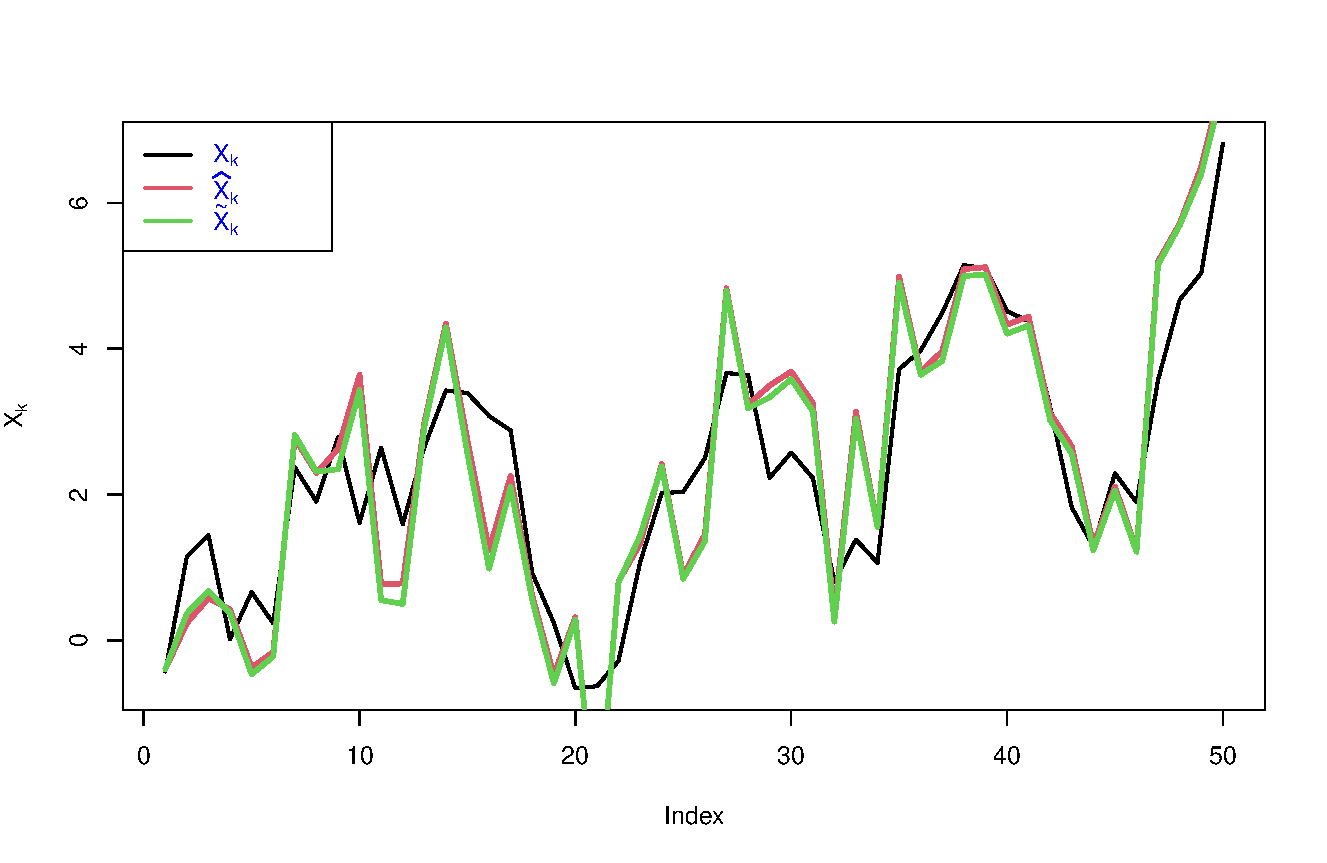
\includegraphics[width=\linewidth]{./ass5.2c-1.pdf}
	\caption{Plot of $X_k$ vs $\hat{X}_k$ vs $\tilde{X}_k$ for $\alpha=1$}
	\label{energydetPSK}
\end{subfigure}

\medskip % create some *vertical* separation between the graphs
\begin{subfigure}{.475\linewidth}
	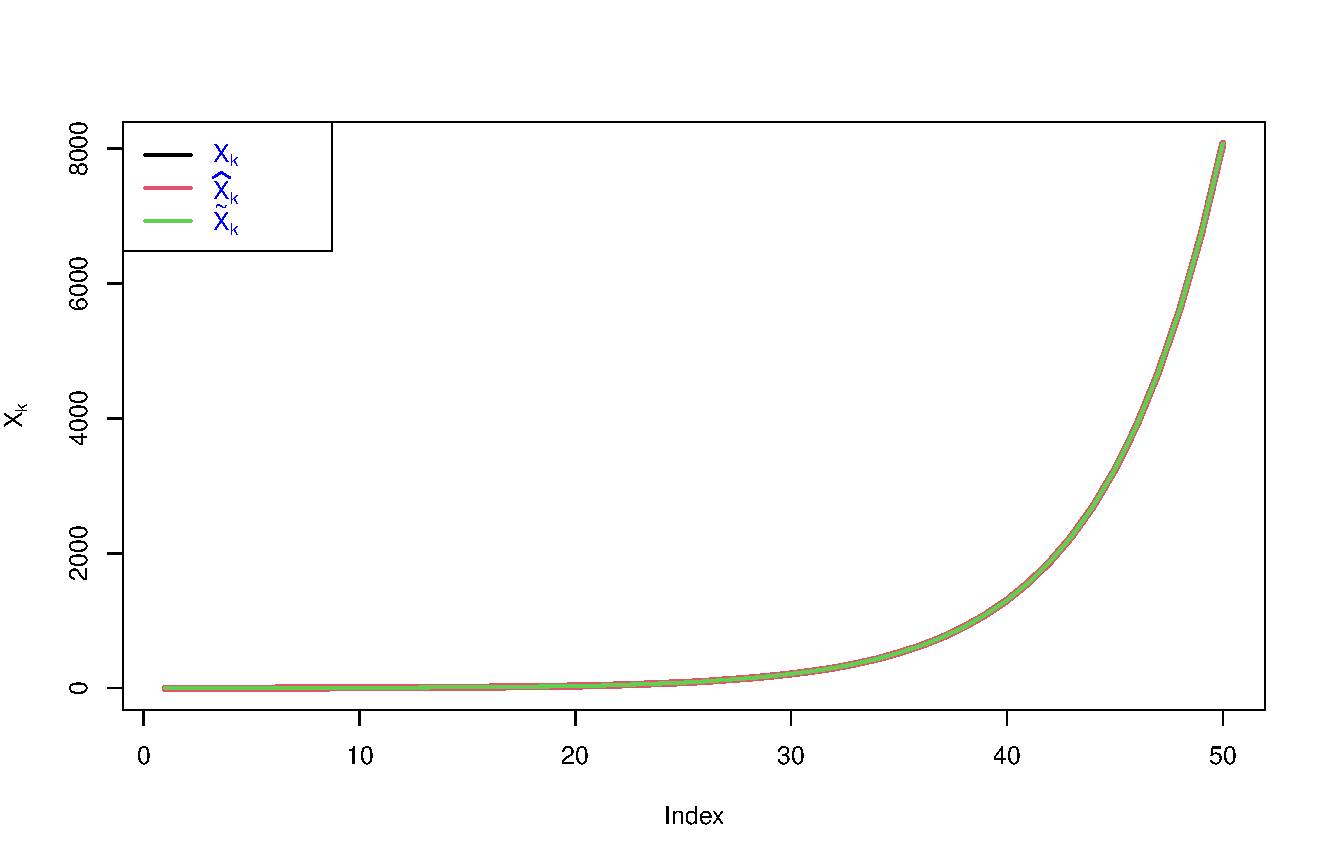
\includegraphics[width=\linewidth]{./ass5.2c-1.2.pdf}
	\caption{Plot of $X_k$ vs $\hat{X}_k$ vs $\tilde{X}_k$ for $\alpha=1.2$}
	\label{velcomp}
\end{subfigure}\hfill % <-- "\hfill"
\begin{subfigure}{.475\linewidth}
	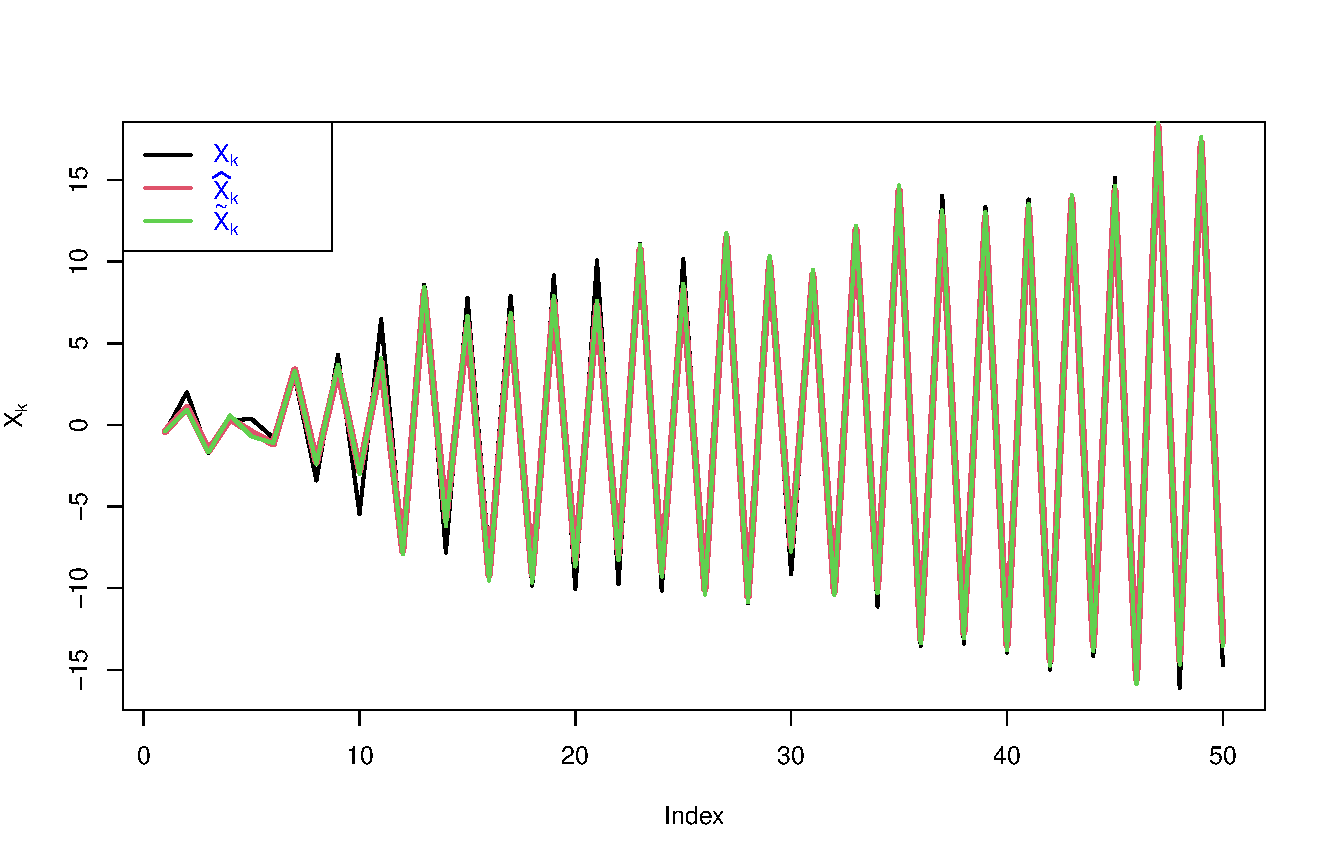
\includegraphics[width=\linewidth]{./ass5.2c--1.pdf}
	\caption{Plot of $X_k$ vs $\hat{X}_k$ vs $\tilde{X}_k$ for $\alpha=-1$}
	\label{estcomp}
\end{subfigure}

\caption{Compared $X_k$ and predicted $\hat{X_k}$ and $\tdX_k$ }
\label{fig:roc}
\end{figure}
\item Here we plot $f_k$ for values $k\in[10]$ with $\alpha=0.8$. Now the conditional distribution $X\mid Y_1,\dots, Y_k$ approaches the distribution $N\lt(0,\frac{\sg2}{1-\alpha^2}\rt)$ for large $k$ and also we notice from the plot that this doesn't depend on the $Y_k$.\newpage

\begin{figure}[hbt!]
	\centering
	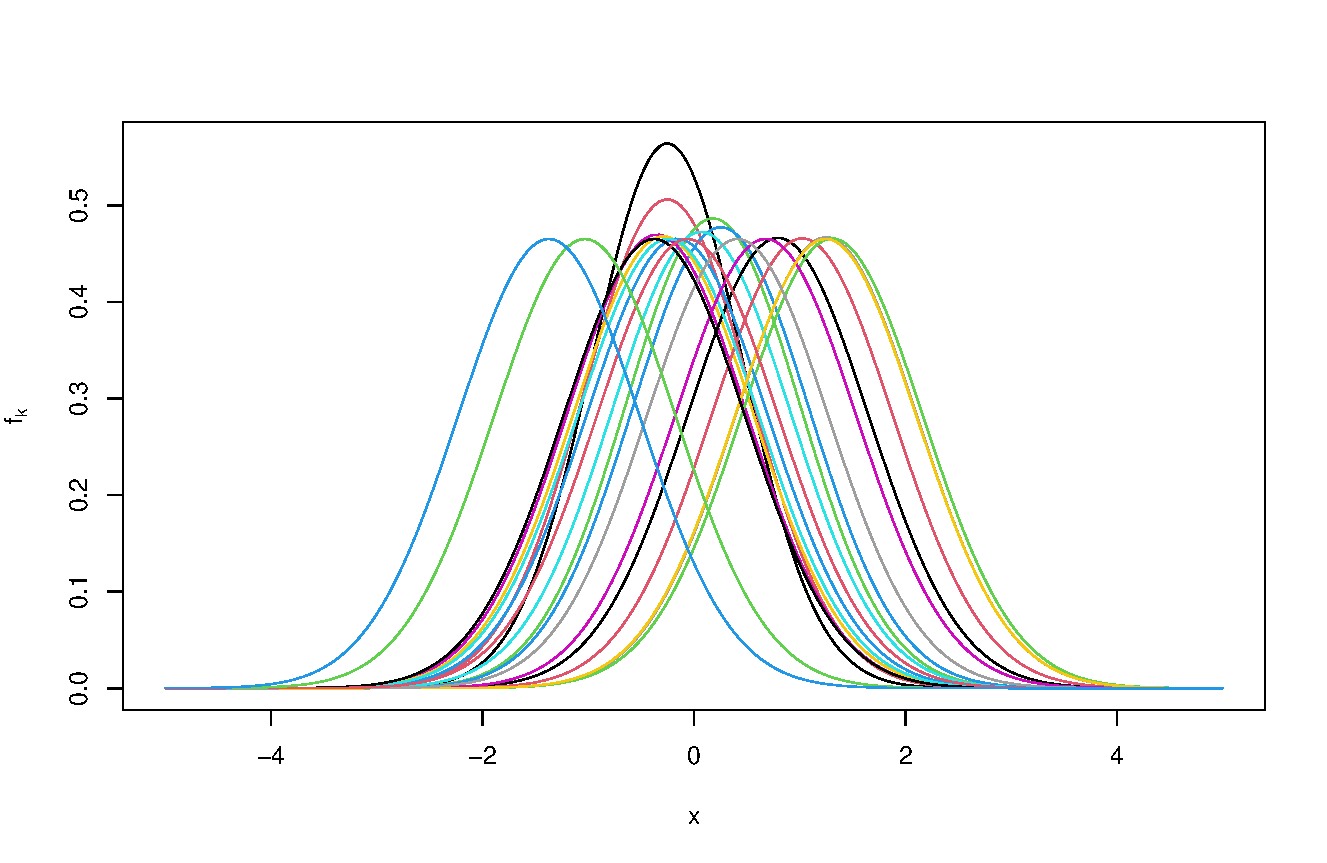
\includegraphics[width=16cm]{./ass5.2d-0.8.pdf}
	\caption{Plot of density $f_k$ of $X_k\mid Y_1,...,Y_k$ for $\alpha=0.8$, $k\in[10]$}
\end{figure}

\item We will induct on $k$. Since $X_1,W_2$ are independent and we have $X_2=\alpha X_1+W_2$ hence $X_2\sim N\lt(0, \alpha^2\sg_{X_1}^2+\sg_W^2\rt)$. Now $X_{k-1}$ and $W_k$ are independent and we have $X_k=\alpha X_{k-1}+W_k$. By inductive hypothesis $X_{k-1}$ follows Gaussian Distribution. Hence $X_k$ also follows Gaussian Distribution. Hence $\bbE[X_k]=0$. Now we have to calculate $\Var[X_k]$.$$\Var[X_k]=\alpha^2\Var[X_{k-1}]+\sg_W^2=\alpha^2(\alpha^2\Var[X_{k-2}]+\sg_W^2)+\sg_W^2=\cdots = \alpha^{2k-2}\sg_{X_1}^2+\sg_W^2\sum_{i=0}^{k-1}\alpha^{2i}$$Therefore $X_k\sim N\lt(0,\alpha^{2k-2}\sg_{X_1}^2+\sg_W^2\sum\limits_{i=0}^{k-1}\alpha^{2i}\rt)$. Hence if $|\alpha|<1$, $\lim\limits_{k\to\infty}\Var[X_k]=\frac{\sg_W^2}{1-\alpha^2}$. Hence as $k\to\infty$, $X_k\to N\lt(0,\frac{\sg_W^2}{1-\alpha^2}\rt)$. Now if $|\alpha|\geq 1$, then as $k\to \infty$, $\alpha^{2k-2}$ diverges. Therefore $\Var[X_k]$ diverges to $+\infty$.\parinn

If $|\alpha|<1$ then $\Var[X_k]=\frac{\sg_W^2}{1-\alpha^2}$. Hence it doesn't depend on $\sg_{X_1}^2$. 
\item Let $\rho_k$ denote the variance of $X_k$. Then we have the formula $$\rho_n=\alpha^2\rho_{n-1}^2+\sg_W^2\quad\text{for } n\geq 2$$Hence we know the behavior of the conditional variance $\sg_k^2$ of ${X_k}$. Hence we know the MMSE of ${X_k\mid Y_1,\dots, Y_k}$ as $k\to \infty$. Now we have $$\sg_k^2=\frac{\rho_k^2\sg_Z^2}{h^2\rho_k^2+\sg_Z^2}=\frac{\sg_Z^2}{h^2+\frac{\sg_Z^2}{\rho_k^2}}$$From the previous part  if $|\alpha|<1$ then $\lim\limits_{k\to \infty}\rho_k=\frac{\sg_W^2}{1-\alpha^2}$ and if $|\alpha|\geq 1$ then as $k\to \infty$, $\rho_k$ diverges to $+\infty$.  Therefore when $|\alpha|<1$, $\lim\limits_{k\to\infty}\sg_k^2=\frac{\sg_Z^2\sg_W^2}{h^2\sg_W^2+(1-\alpha^2)\sg_Z^2}$ and when $|\alpha|\geq 1$ we have $\lim\limits_{k\to\infty}\sg_k^2=\frac{\sg_Z^2}{h^2}$.
\end{enumerate}
}

%%%%%%%%%%%%%%%%%%%%%%%%%%%%%%%%%%%%%%%%%%%%%%%%%%%%%%%%%%%%%%%%%%%%%%%%%%%%%%%%%%%%%%%%%%%%%%%%%%%%%%%%%%%%%%%%%%%%%%%%%%%%%%%%%%%%%%%%
% Problem 3
%%%%%%%%%%%%%%%%%%%%%%%%%%%%%%%%%%%%%%%%%%%%%%%%%%%%%%%%%%%%%%%%%%%%%%%%%%%%%%%%%%%%%%%%%%%%%%%%%%%%%%%%%%%%%%%%%%%%%%%%%%%%%%%%%%%%%%%%


\begin{problem}{%problem statement
    }{p3% problem reference text
    }
For the system in \hyperref[p:p2]{Problem \ref{p:p2}} derive a recursive algorithm for computing the one-step ahead estimator: $\bbE[{X_k\mid Y_1,Y_2,\dots, Y_k,Y_{k+1}}]$. This means we can look ahead one step to estimate the state.
\end{problem}
\solve{
We have $Y_{k+1}=hX_{k+1}+W_{k+1}$. and $X_{k+1}=\alpha X_k+Z_k$. Therefore combining these two we have $$Y_{k+1}=\alpha hX_k+(hW_k+Z_{k+1})$$Now take $T_k=hW_k+Z_{k+1}$. Then $T_k\sim N(0,h^2\sg_W^2+\sg_Z^2)$. Now denote $Y_1^k=(Y_1,\dots, Y_k)$ and denote $y_1^k=(y_1,\dots, y_k)$. Then we have  $$f\st_{X_k\mid Y^{K+1}_1}(x\mid y_1^{k+1})=\frac{f\st_{Y_{k+1}\mid X_k,Y^{K}_1}(y_{k+1}\mid x_k,y_1^{k})}{f\st_{Y_{k+1}\mid Y^{K}_1}(y_{k+1}\mid y_1^{k})}f_{X_k\mid Y_1^k}(x_k\mid y_1^k)$$Combining this with $\alpha hX_k+(hW_k+Z_{k+1})$ we can write $$\bbE[X_k\mid Y_1^{k+1}]=h\alpha \bbE[X_{k-1}\mid Y_1^k]$$
}



\end{document}
